%!TEX root = ./main.tex


\section{Intro}
\addtocounter{minutes}{2}
\begin{frame}%
	\frametitle{Intro}%
	%\framesubtitle{}
    Initiatief van studenten
	\vspace{0.2cm}
	
   	\centering%
    \begin{minipage}{0.30\linewidth}%
        \centering%
        \noindent
\includegraphics[width=\linewidth]{res/arno} \\%
        \footnotesize Arno Deceuninck \strut%
    \end{minipage}
    \begin{minipage}{0.30\linewidth}%
        \centering%
		
\includegraphics[width=\linewidth]{res/you} \\%
        \footnotesize Jij? \strut%
    \end{minipage}
    \begin{minipage}{0.30\linewidth}%
        \centering%
		
\includegraphics[width=\linewidth]{res/mateo} \\%
        \footnotesize Mateo Sierens \strut%
    \end{minipage}
      	
    \begin{minipage}{0.30\linewidth}%
        \centering%
		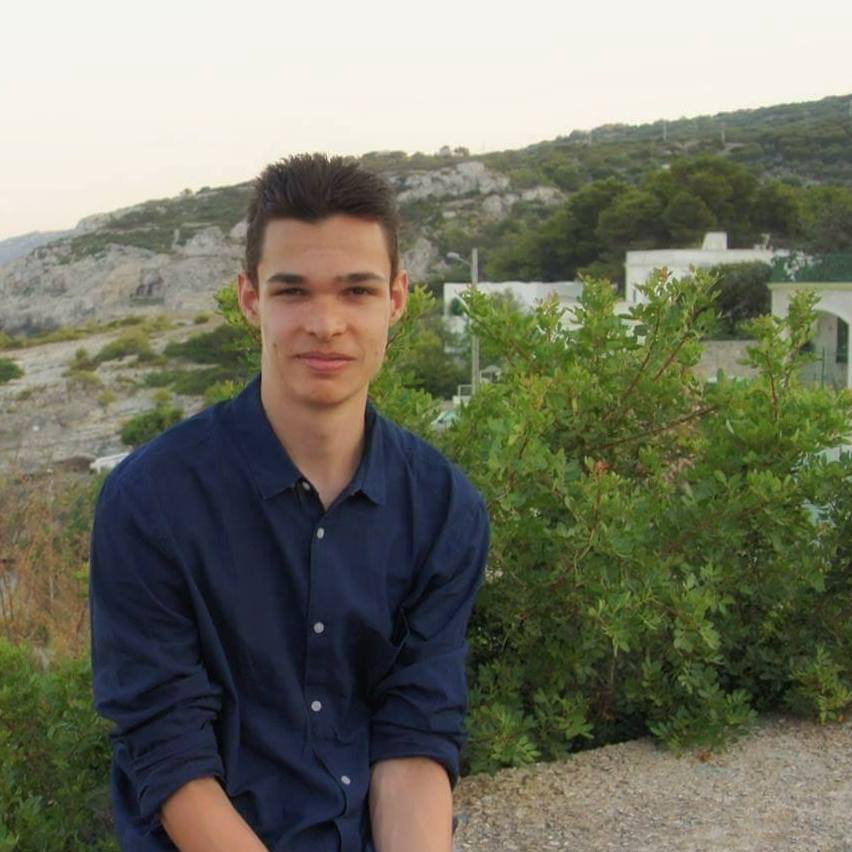
\includegraphics[width=\linewidth]{res/stijn} \\%
        \footnotesize Stijn Rosaer \strut%
    \end{minipage}
    \begin{minipage}{0.30\linewidth}%
        \centering%
		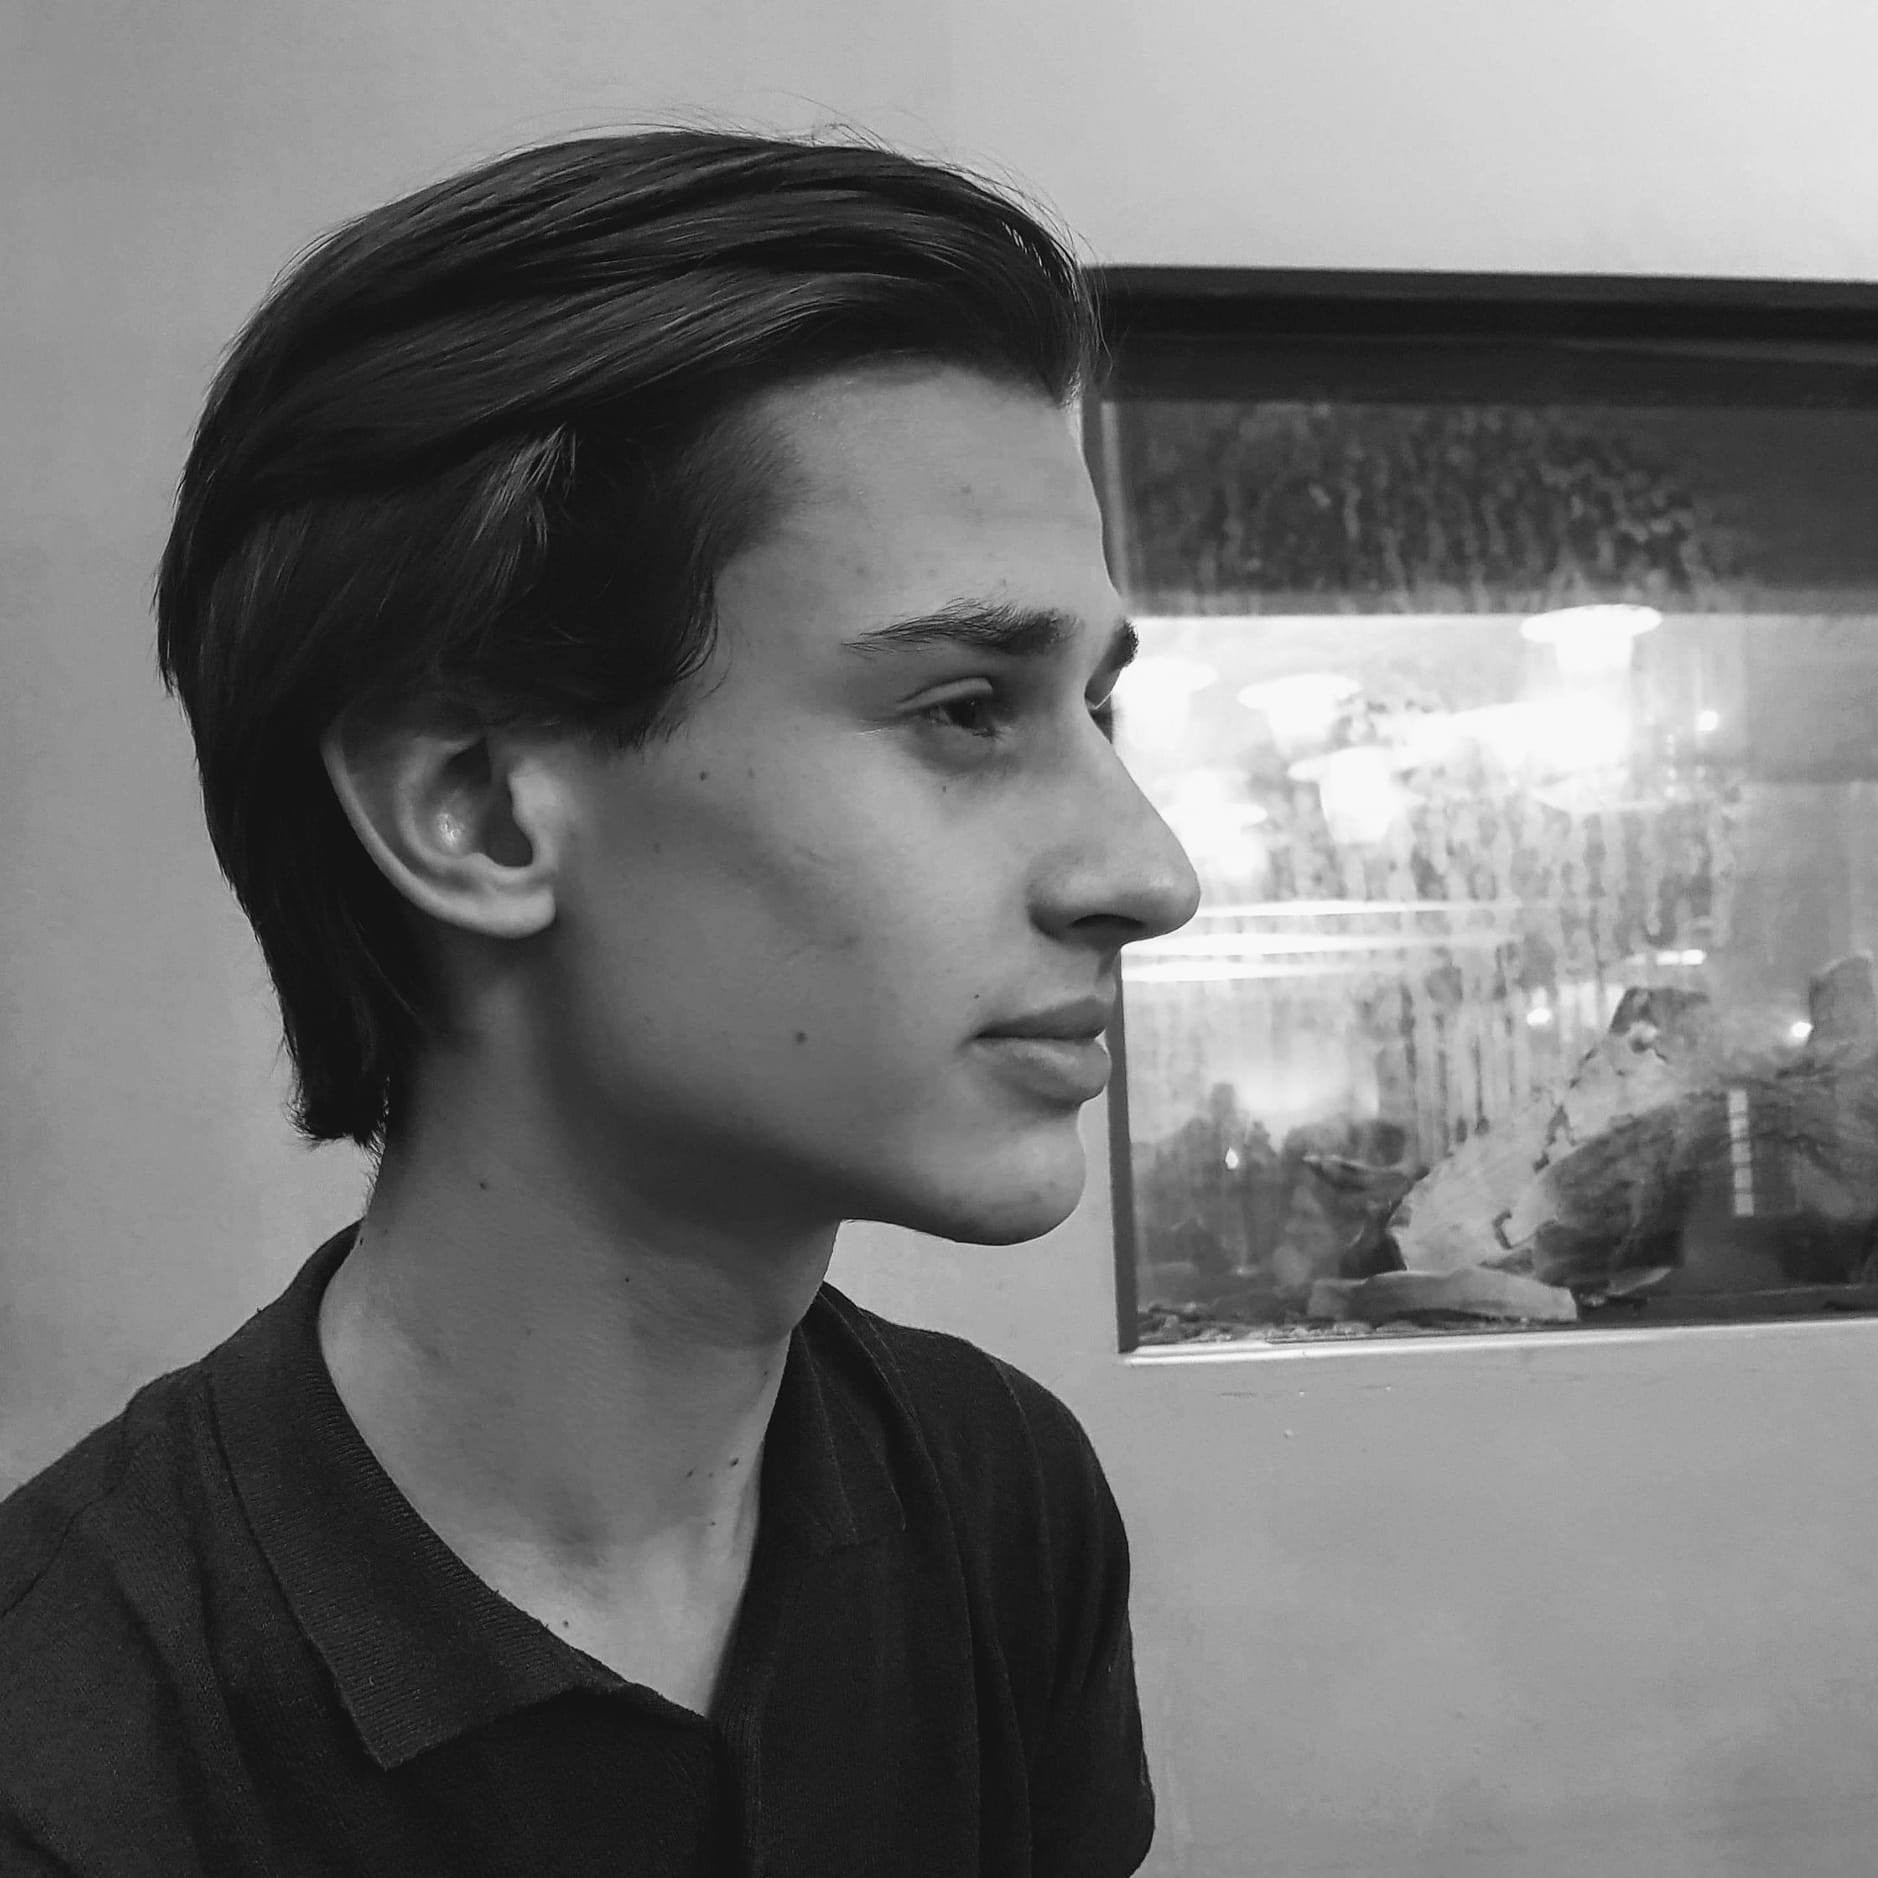
\includegraphics[width=\linewidth]{res/senne} \\%
        \footnotesize Senne Rosaer \strut%
    \end{minipage}
    \begin{minipage}{0.30\linewidth}%
		\centering%
		
\includegraphics[width=\linewidth]{res/toon} \\%
		\footnotesize Toon Meynen \strut%
    \end{minipage}
\end{frame}  
   
    
\section{Planning}
\addtocounter{minutes}{3}
\begin{frame}
	\frametitle{Planning}
    \includeSchedule
    
	% NOTE: Volgende sessie:  Dual boot $->$ USB stick en laptop

\end{frame}

\section{WINAK}
\begin{frame}
	\frametitle{WINAK}
	\framesubtitle{\textbf{W}iskunde \textbf{I}nformatica \textbf{Na}tuurkunde \textbf{K}ring}
    
    \begin{itemize}
        \item\link{https://www.facebook.com/groups/2422547801192952/}{Facebook Groep}
        \item\link{http://tuyaux.winak.be/}{Tuyaux}
        \item Lidkaart
        \item Mentoren
        \begin{itemize}
           	\item\link{https://www.facebook.com/ruben.lauwereys} {Ruben (Wiskunde)}
           	\item\link{https://www.facebook.com/ilias.elattabi} {Ilias (Fysica)}
			\item\link{https://www.facebook.com/arno.deceuninck} {Arno (Informatica)}
		\end{itemize}
		\item Doop
        \item\link{https://www.facebook.com/events/467170507207722/}{Openings Cafe Avond}
        
	\end{itemize}

\end{frame}
    
%     \section{Blackboard \& SiSa}
% 	\begin{frame}
% 		\frametitle{Blackboard}
% 		\framesubtitle{https://blackboard.uantwerpen.be}
%         \begin{itemize}
%         \item Facebook van de universiteit
%           \begin{itemize}
%             \item Updates
%             \item Projecten
%             \item Oefeningen
%           \end{itemize}
% 		\end{itemize}
% 	\end{frame}
	
% 	\begin{frame}
% 		\frametitle{SiSa}
% 		\framesubtitle{https://sisastudent.uantwerpen.be}
%         \begin{itemize}
%           \item Administratie van de universiteit
%           \begin{itemize}
%             \item Inschrijven
%             \item Lessenrooster
%             \item Rekeningen
%           \end{itemize}
% 		\end{itemize}
% 	\end{frame}
    
\section{Email \& Lessenrooster}
\begin{frame}
	\frametitle{Email}
	\framesubtitle{\url{https://mail.student.uantwerpen.be}}
    \begin{center}
       	\tcbox[colback=white, colframe=darkblue]{
           	\parbox{7.5cm}{
              \centering
              s019xxxx@ad.ua.ac.be OF \\
              voornaam.achternaam@student.uantwerpen.be
            }
        }
    \end{center}
   	\textbf{IMAP (inkomend)}
    \begin{tabularx}{\linewidth}{rX}
      Server name & outlook.office365.com \\
      Port & 993 \\
      Encryption & SSL \\
	\end{tabularx} \vspace{0.5cm}
    
	\textbf{SMTP (uitgaand)}
    \begin{tabularx}{\linewidth}{rX}
      Server name & smtp.office365.com \\
      Port & 587 \\
      Encryption & STARTTLS \\
	\end{tabularx} \vspace{0.5cm}
    
   % NOTE: mogelijk dient u poort 143 te gebruiken bij de IMAP instellingen, wanneer het niet meteen lukt om met bovenstaande gegevens uw e-mail binnen te halen.
\end{frame}
    
\begin{frame}
	\frametitle{Lessenrooster}
	%\framesubtitle{}
	
	\begin{itemize}
		\item<1-> SiSa: \link{https://sisastudent.uantwerpen.be}{https://sisastudent.uantwerpen.be}
		\item<1-> ``Rooster''
		\item<2-> ``abonneer op rooster''
	\end{itemize}
	
	\only<1-2>{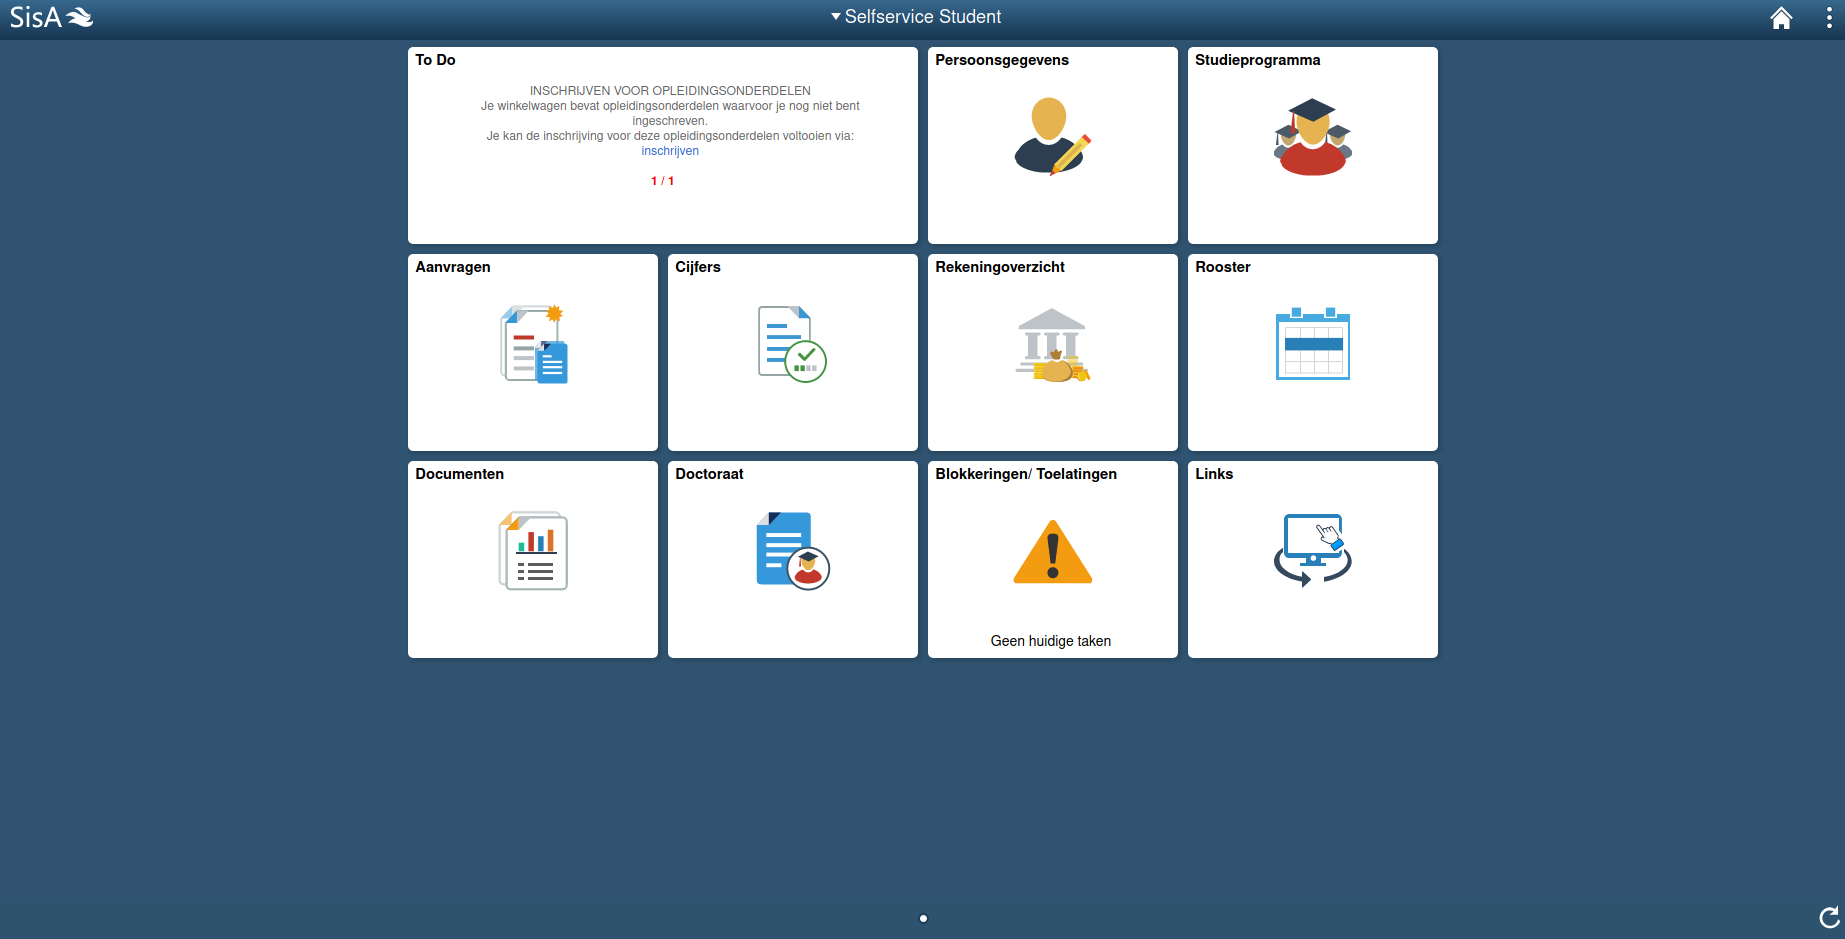
\includegraphics[width=\linewidth]{res/sisa_rooster_1}}
	\only<3>{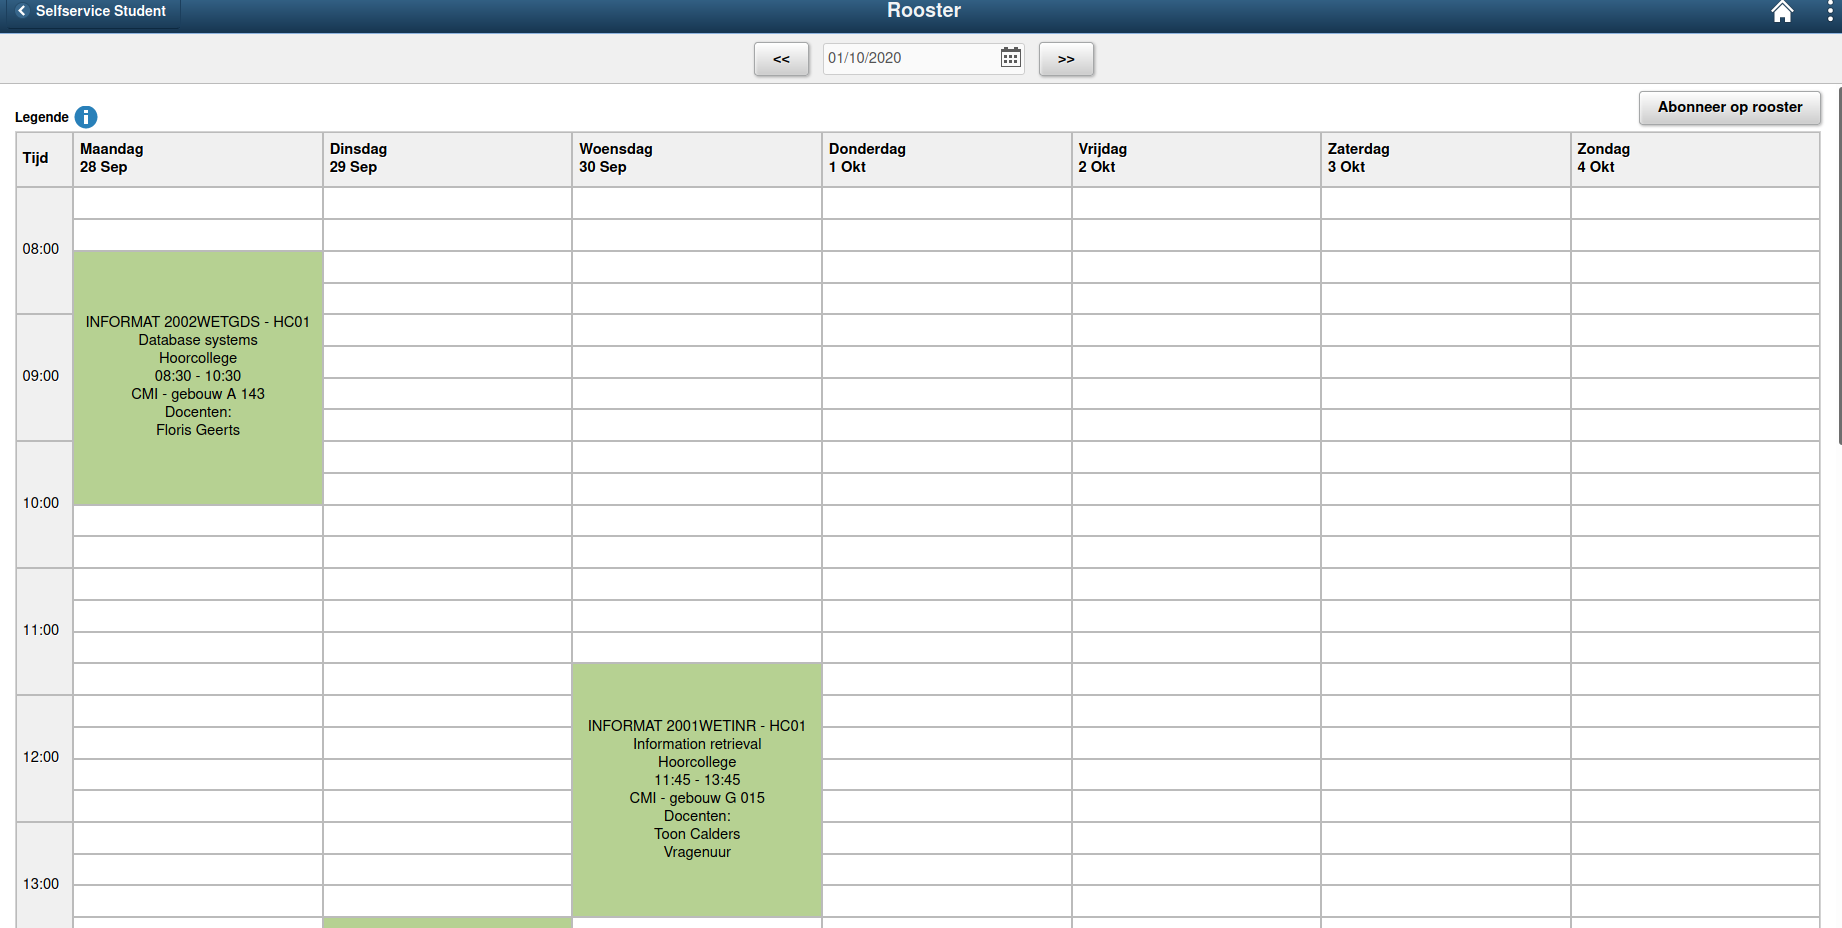
\includegraphics[width=\linewidth]{res/sisa_rooster_2}}
	\visible<4>{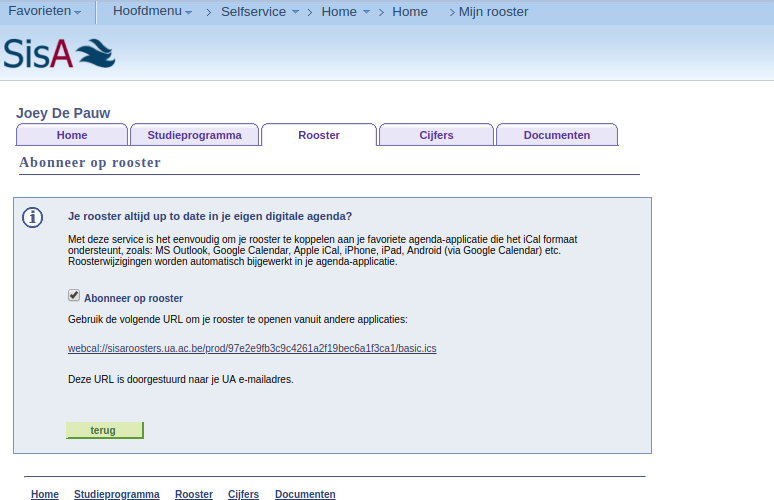
\includegraphics[width=\linewidth]{res/sisa_rooster_3}}
    
\end{frame}

\section{Cursusdienst}
\begin{frame}[allowframebreaks=10]
	\frametitle{Cursusdienst}
	%\framesubtitle{}
    \vspace{0.5cm}
    
    Tips:
    \begin{itemize}
        \item Verplicht $\neq$ verplicht verplicht
        \item Cursussen zeker kopen
        \item Handboeken ter referentie
        \item Ga op tijd je boeken halen, soms zijn ze uitverkocht en bestellen duurt even
	\end{itemize}
    
	% NOTE:
	% Verplicht = sterk aangeraden door prof
	% Cursussen: relatief goedkoop, soms op examens gebruiken
	% Handboeken: duurder, meer achtergrond info, kan handig zijn

    
    \framebreak
    \begin{figure}
       	\centering
        \vspace*{0.02cm}
        \textbf{Campus Groenenborger} \\
        \vspace{0.3cm}
       	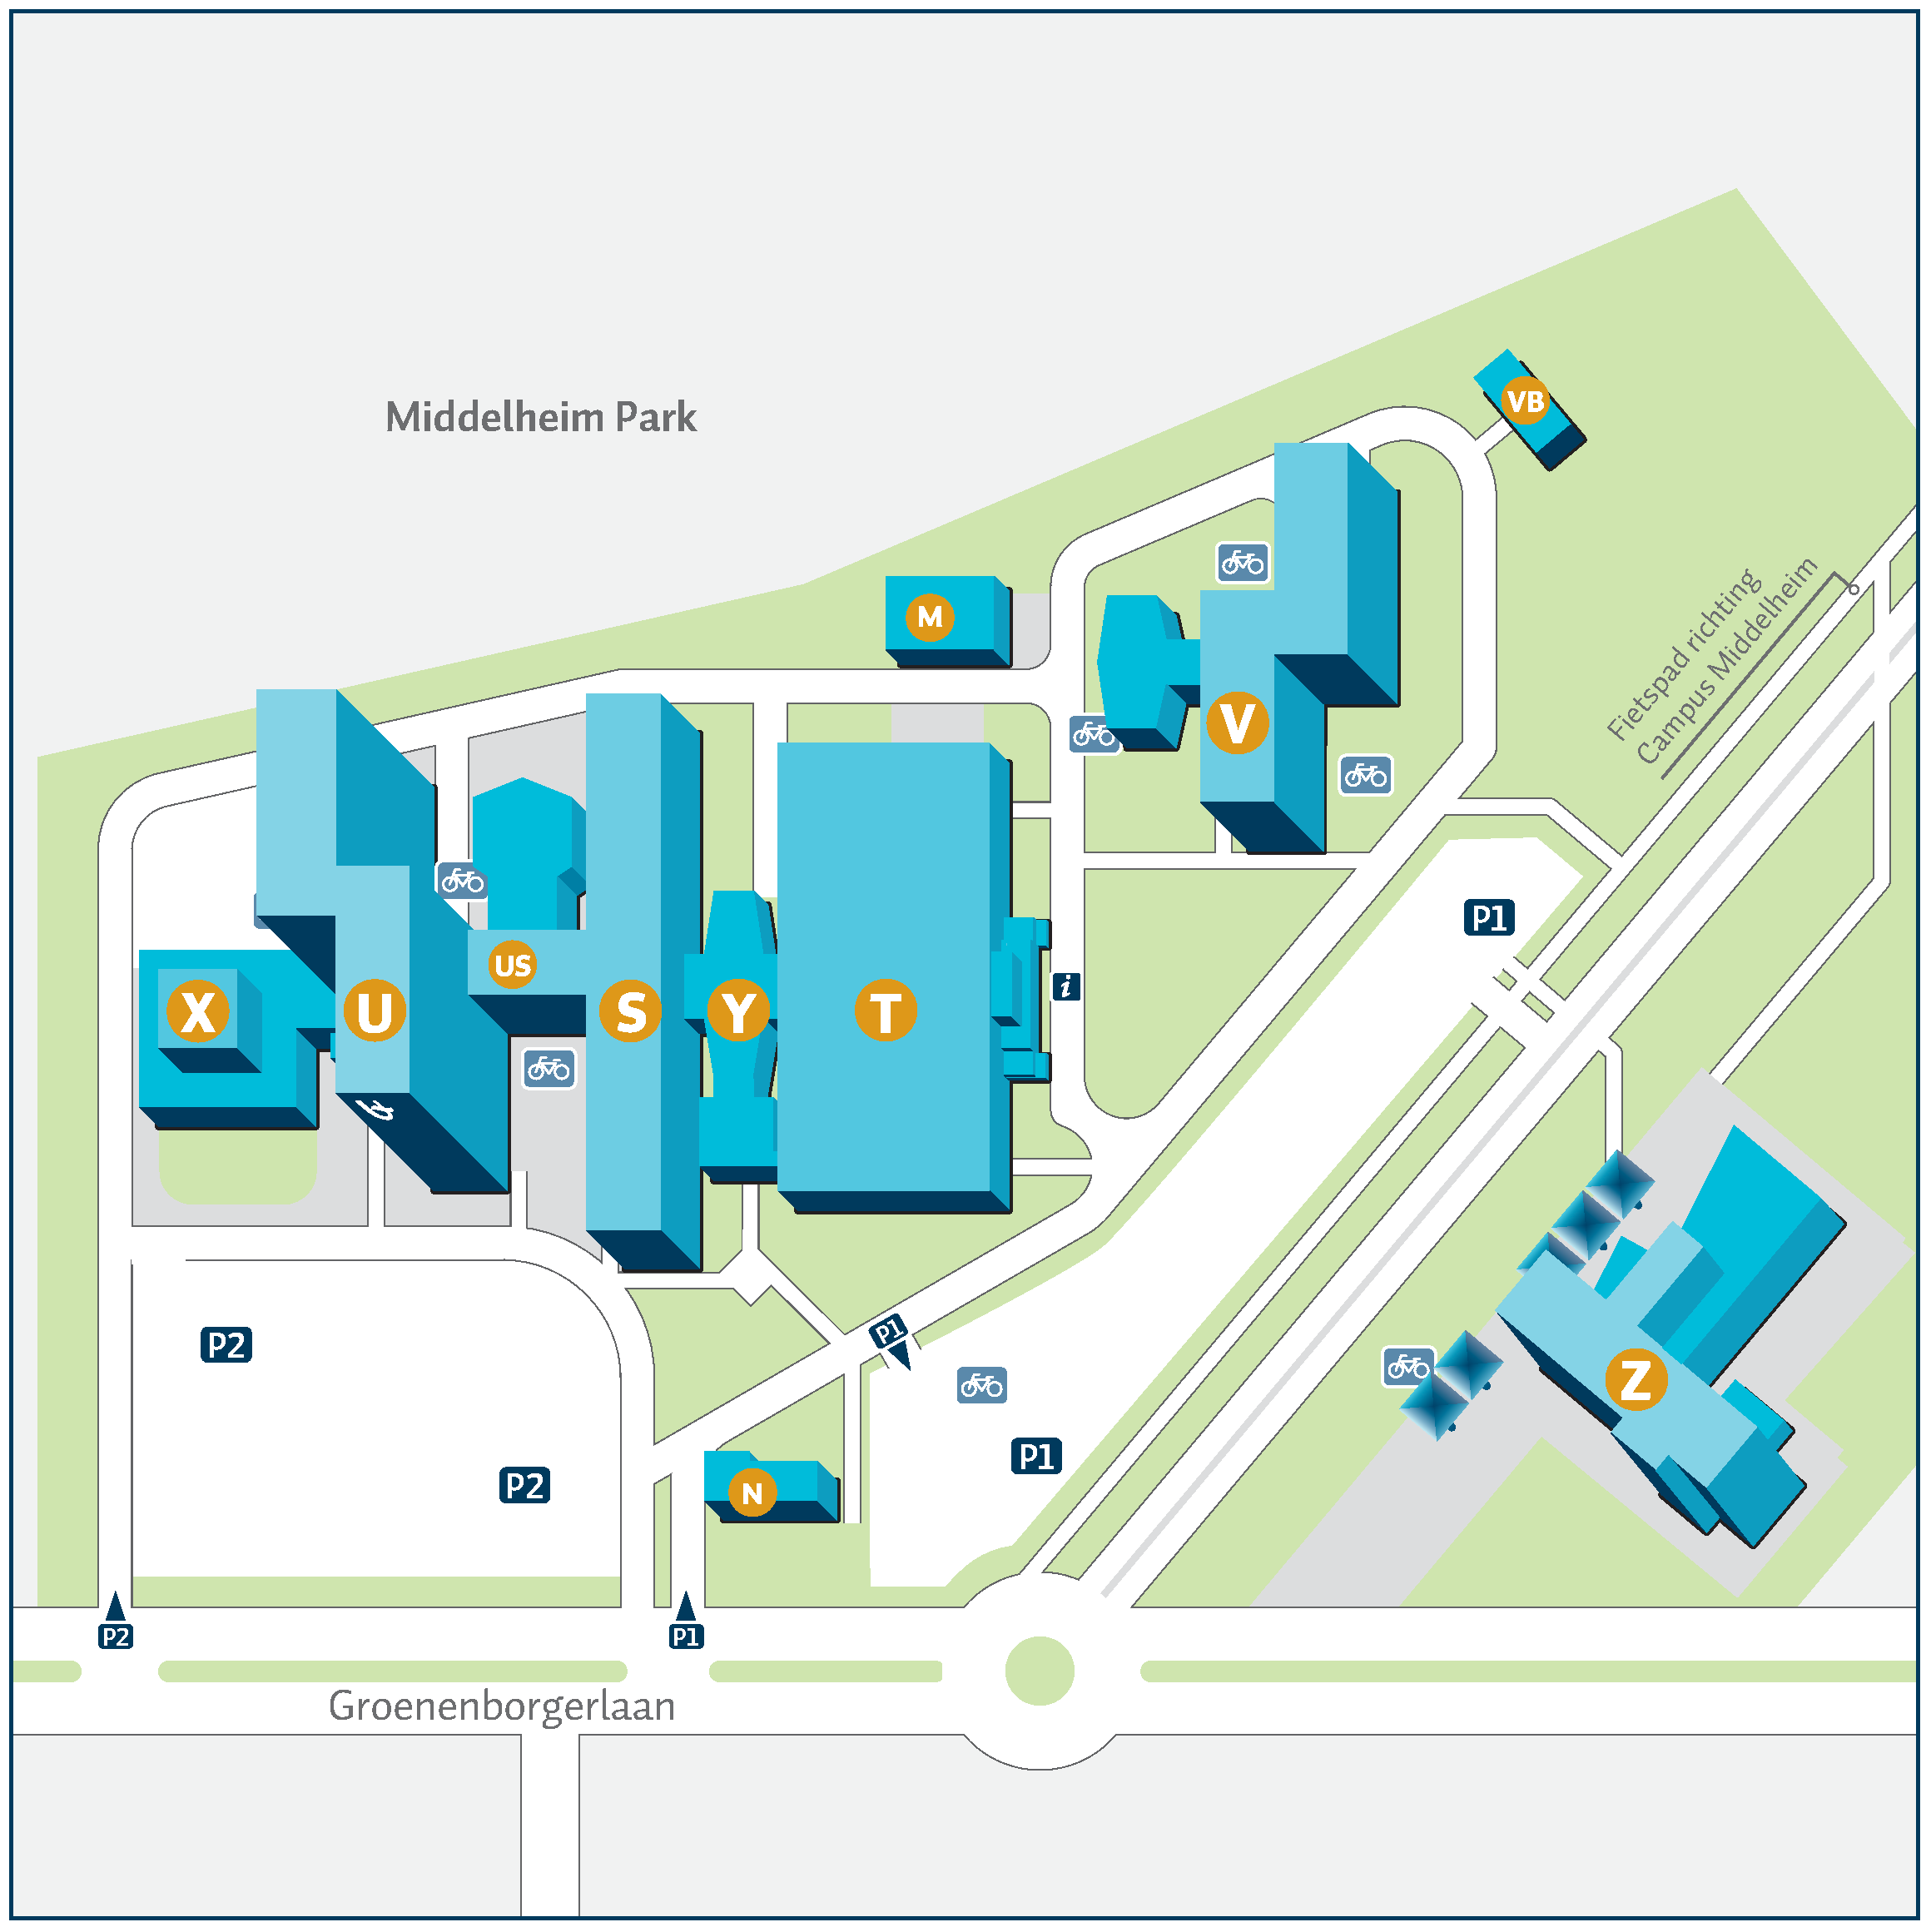
\includegraphics[width=0.65\linewidth]{res/CGB}
    \end{figure}
    \framebreak
    \begin{figure}
       	\centering
        \vspace*{0.02cm}
        \textbf{Cursusdienst Campus Groenenborger U027} \\
        \vspace{0.3cm}
      	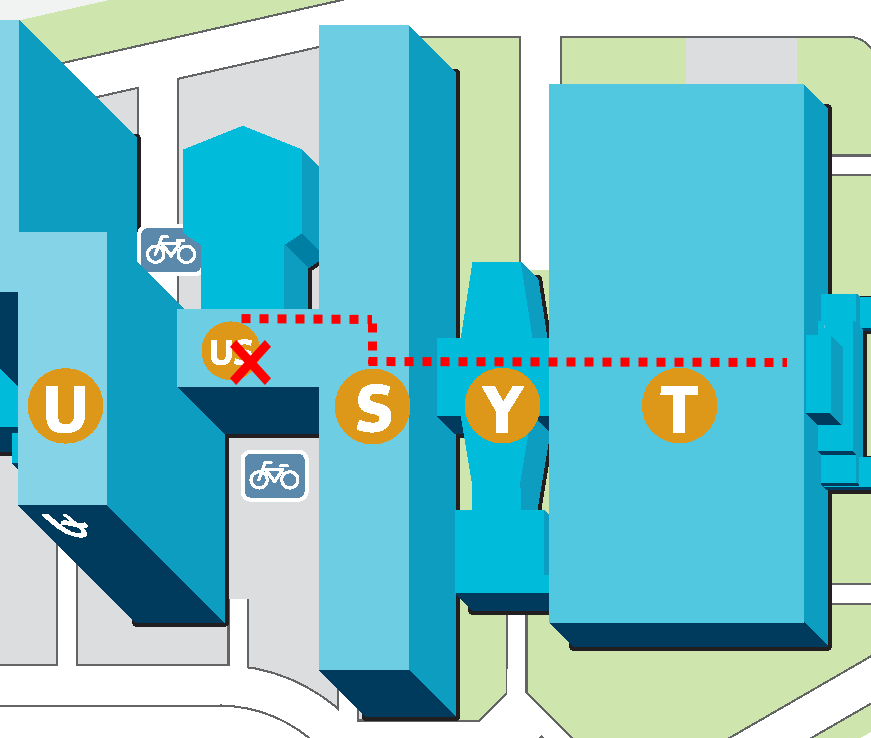
\includegraphics[width=0.8\linewidth]{res/CGB_CD_small}
    \end{figure}
\end{frame}

\section{Cursussen}
\begin{frame}[allowframebreaks=10]
	\frametitle{Cursussen}
	\link{https://www.cursusdienst.be}{Cursusdienst}
	
	\begin{itemize}
		\item Kijk vooraf welke cursussen beschikbaar zijn
		\item Online bestellen mogelijk
	\end{itemize}
	
	\framebreak

	\centering
    \vspace*{0.02cm}
    \textbf{Selectie} \\
    \vspace{0.6cm}	
	
	\begin{tabularx}{\linewidth}{rX}
	  Instelling/Campus & UA: Campus Groenenborger/Middelheim\\
	  Faculteit/Departement & Wetenschappen\\
	  Bachelor/Master & Wetenschappen\\
	  Traject & Informatica\\
	  Jaar/Studiegroep & Bachelor Modeltraject 1 (1e jaar)\\
	\end{tabularx} \vspace{0.5cm}
	
\end{frame}

%\begin{frame}[allowframebreaks=10]
%	\frametitle{Printen}
%	% framesubtitle{}
%    
%    \link{https://www.uantwerpen.be/nl/bibliotheek/diensten/faciliteiten/ter-plaatse/printen-kopieren-scannen/}{Website UA - Printen}
%    \vspace{0.5cm}
%    
%    \begin{enumerate}
%        \item Laad je studentenaccount online op (min \euro5 - max \euro50)
%        \item Printen
%    \end{enumerate}
%
%\end{frame}

\section{Rondleiding \& Receptie}
\begin{frame}
	\frametitle{Rondleiding \& Receptie}
	\framesubtitle{Sponsored by WINAK}
    \begin{itemize}
    	\item Super geheime automaat gebouw A
       	\item Gebouw G
	    \item Computerlokaal M.G.025
        \item Leercentrum ``De Parabool''
        \item PC Labo
        \item Free Drinks
	\end{itemize}
\end{frame}
